\chapter{Special Distributions} \label{ch:commondistribution}

Commonly seen special distributions, both discrete and continuous, are introduced here. Some of them are very useful in statistics analysis and are introduced in more details in later part of the notebook.

\section{Bernoulli and Binomial}

\textit{Bernoulli distribution} is a discrete probability distribution of random variable $X$ that can take only 2 values, $0$ or $1$. The probability of $X$ taking $1$ is denoted by $p$, while $0$ is $q=1-p$ as shown below.
\begin{eqnarray}
  && f(x) = P(X=x) = \left\{\begin{array}{cc}
                           p & x=1 \\
                           q & x=0
                         \end{array}\right. \nonumber
\end{eqnarray}
subject to $0\leq p \leq 1$, $0\leq q \leq 1$ and $p+q=1$. Each test is also called a Bernoulli trail.

The expectation, variance, skewness and excess kurtosis of the distribution are $p$, $pq$, $\dfrac{q-p}{\sqrt{pq}}$ and $\dfrac{1-6pq}{pq}$, respectively.

Run Bernoulli trails repeatedly. Each bernoulli trail has a probability of $p$ to take value $1$, and $q=1-p$ to take value $0$. The test is carried out $n$ times. The number of the tests with outcome $1$ is a discrete random variable $0\leq X \leq n$. In this case, $X$ follows \textit{binomial distribution}, whose probability function is given by
\begin{eqnarray}
  f(x) &=& P(X=x) \nonumber \\
  &=& \left(\begin{array}{c}
              n \\
              x
            \end{array}\right)p^x(1-p)^{n-x} \nonumber \\
  &=& \dfrac{n!}{x!(n-x)!}p^x(1-p)^{n-x}
\end{eqnarray}

Bernoulli distribution can be taken as a special case of binomial distribution with $n=1$, $x=1$. The expectation, variance, skewness and excess kurtosis of the distribution are $np$, $npq$, $\dfrac{q-p}{\sqrt{npq}}$ and $\dfrac{1-6pq}{npq}$, respectively.

Binomial distribution is naturally a verification of CLT on Bernoulli trail. According CLT, when $n$ is large, binomial distribution should approach normal distribution.

Binomial distribution can be extended to \textit{multinomial distribution}, where instead of a single event $A$ happening with probability $p$ or not happening with probability $q$, s.t. $p+q=1$, consider multiple events $A_1$, $A_2$, ..., each with probability $p_1$, $p_2$, ..., respectively, s.t. $p_1+p_2+\ldots+p_m=1$. Consider a total of $n$ tests. The number of $A_1$ occurring is a random variable $X_1$, event $A_2$, $X_2$, and so on. Multinomial distribution studies the probability of
\begin{eqnarray}
  P(X_1=x_1, X_2=x_2,\ldots, X_m = x_m) &=& \dfrac{n!}{x_1!x_2!\ldots x_m!}p_1^{x_1}p_2^{x_2}\ldots p_m^{x_m} \nonumber \\
  \textup{s.t.} && \sum x_i = n \nonumber
\end{eqnarray}

Do distinguish binomial distribution with \textit{hypergeometric distribution}. Binomial distribution is used to model ``sampling with replacement'' process: each Bernoulli trail backing up the binomial distribution is i.i.d. and one's result is not affected by its previous trails. Consider picking up a marbles from a bag containing mixture of red and blue marbles whose numbers are given by $r$ and $b$ respectively. Repeat the test $n$ times. After each test, put the marble back to the bag. The number of blue marbles collected is a random variable $X$ that follows binomial distribution
\begin{eqnarray}
f(x) &=& \left(\begin{array}{c}
                        n \\
                        x
                      \end{array}\right)\left(\dfrac{b}{b+r}\right)^x\left(\dfrac{r}{b+r}\right)^{n-x} \nonumber \nonumber
\end{eqnarray}

On the other hand, if after each test the marble is not returned to the bag, it becomes a hypergeometric distribution and the probability follows
\begin{eqnarray}
f(x) = P(X=x) = \dfrac{\left(\begin{array}{c}
                               b \\
                               x
                             \end{array}\right)\left(\begin{array}{c}
                                                       r \\
                                                       n-x
                                                     \end{array}\right)}{\left(\begin{array}{c}
                                                                                 b+r \\
                                                                                 n
                                                                               \end{array}\right)} \nonumber
\end{eqnarray}
with $\textup{max}(0, n-r) \leq x \leq \textup{min}(n, b)$.

When $b$, $r$ are far larger than $n$, the hypergeometric distribution can be approximated by the binomial distribution. When $b$ and $r$ approaches infinity with constant ratio $b/(b+r)$ and $r/(b+r)$, hypergeometric distribution converges to binomial distribution.

\section{Normal Distribution}

Normal distribution, also known as Gaussian distribution, is a continuous distribution. It is one of the most widely used assumption of random noise. One of the explanations is given as follows. Many measurements such as sensor readings are in fact aggregated values. For example, consider a sensor whose reading refreshes at $1Hz$. Behind the screen, it might be sampling the signal at $1000Hz$, and the reading is the average of every $1000$ samples. According to CLT, the reading shall follow normal distribution.

We will discuss single normal distribution first, followed by joint multivariate normal distribution.

\subsection{Single Normal Distribution}

The PDF of the normal distribution is given by
\begin{eqnarray}
  f(x) &=& \dfrac{1}{\sigma\sqrt{2\pi}}e^{-\dfrac{(x-\mu)^2}{2\sigma^2}} \nonumber
\end{eqnarray}
where $\mu$, $\sigma^2$ are the mean and variance of the distribution respectively. The skewness and excess kurtosis of normal distribution are zero.

Let $X$ be a random variable following normal distribution with mean $\mu$ and variance $\sigma^2$. This can be denoted by $X\sim\mathcal{N}(\mu, \sigma^2)$. Let $Z=\dfrac{X-\mu}{\sigma}$, and $Z$ would be a standard normal distribution with mean $0$ and variance $1$.

For a random variable $X$ following normal distribution, the probabilities of its value falling between $\pm \sigma$, $\pm 2\sigma$ and $\pm 3\sigma$ are $0.6827$, $0.9545$ and $0.9973$ respectively. In statistics, sometimes we will take samples with residuals larger than $|3\sigma|$ as outliers.

\subsection{Multivariate Normal Distribution}

Multivariate normal distribution describes a vector of random variables $X = \left[X_1, \ldots, X_m\right]$ that follows joint normal distribution. The joint PDF is given by
\begin{eqnarray}
  f(x) &=& \dfrac{1}{\sqrt{(2\pi)^m|\Sigma|}}e^{-\dfrac{(x-\mu)^T\Sigma^{-1}(x-\mu)}{2}} \nonumber
\end{eqnarray}
where $\mu \in \mathbb{R}^m$ is the mean of $x$ and $\Sigma \in \mathbb{R}^{m\times m}$ the covariance matrix. The off diagonal elements in $\Sigma$ describes the correlation of elements in $X$. The $|\Sigma|$ is the determinant of $\Sigma$.

\section{Poisson Distribution}

Poisson distribution is a discrete probability distribution that takes non-negative integer values $0$, $1$, $2$, $\ldots$.

The probability function of poisson distribution is given by
\begin{eqnarray}
  f(x) = P(X=x) = \dfrac{\lambda^xe^{-\lambda}}{x!} \nonumber
\end{eqnarray}
where $\lambda >0$ is the shape parameter as shown in Fig. \ref{fig:poisson_pmf}.
\begin{figure}
	\centering
	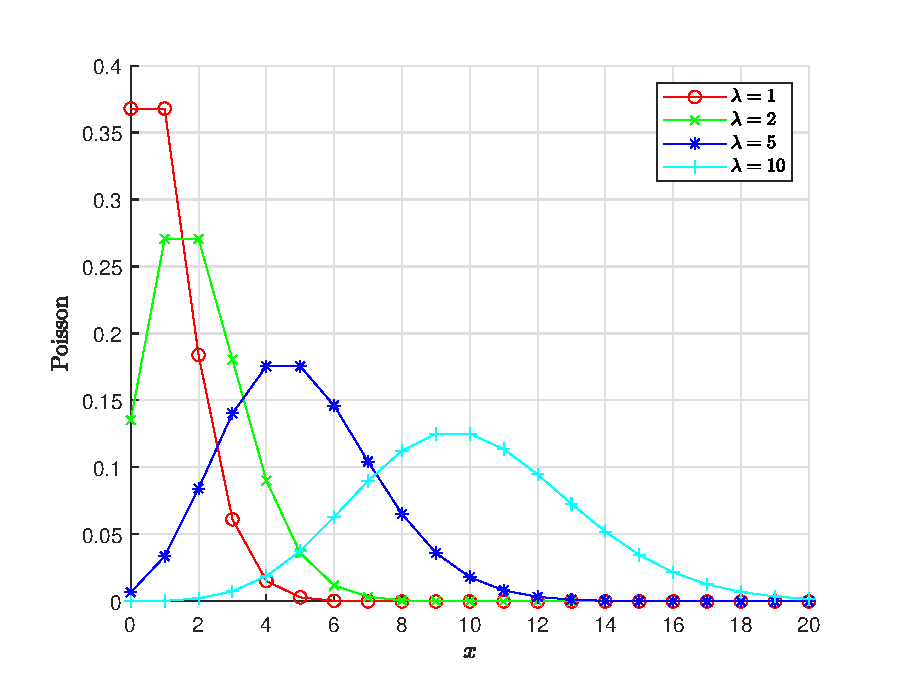
\includegraphics[width=250pt]{chapters/ch-commonly-seen-distributions/figs/poisson_pmf.eps}
	\caption{Poisson distribution with different $\lambda$.} \label{fig:poisson_pmf}
\end{figure}

Notice that The sum of two Poisson distribution with shape parameters $\lambda_1$ and $\lambda_2$ is also Poisson distribution with $\lambda = \lambda_1 + \lambda_2$.

Poisson distribution is often used to describe the probability of an event happening in the given window, for example, the number of times a machine fails in a given length of duration (say one year), assuming each failure is independent from another. 

Binomial distribution is closely connected with Poisson distribution. Poisson distribution can be taken a limiting case of binomial distribution when $n\rightarrow\infty$, $p\rightarrow 0$ is small, and $\lambda = np$ a decent value. A demonstration is given in Fig. \ref{fig:poisson_vs_b}.
\begin{figure}
	\centering
	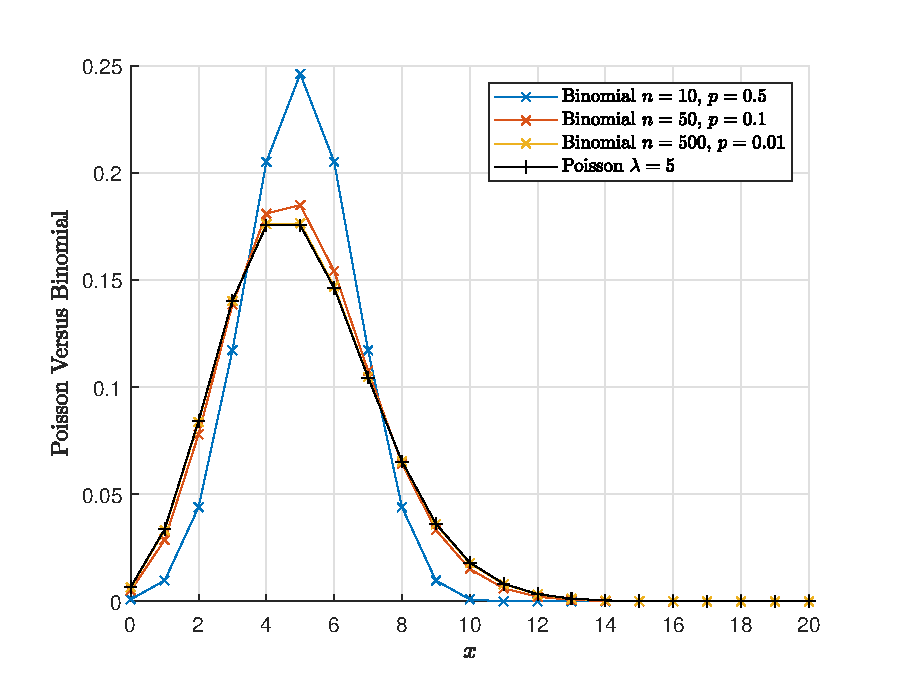
\includegraphics[width=250pt]{chapters/ch-commonly-seen-distributions/figs/poisson_vs_b.eps}
	\caption{Poisson distribution approximation using binomial distribution.} \label{fig:poisson_vs_b}
\end{figure}

An intuitive explanation is given using the following example. Consider studying the number of failure of a machine in one year. In each second, the machine has a failure rate of $p$, which of course is very small. The total number of seconds in a year is $31,536,000$, which is associated with the number of trails. Therefore, the number of failure of the machine in a year can be approximately described by binomial distribution with $x=31536000$. The underlying assumption is that the machine can either pass or fail every second, and it can fail only once per second.

Another example of Poisson distribution is the number of visitors of a website in a given period of time. Each internet user has a small probability $p$ to visit the shopping site. The total number of internet users is $n$ which is a large number. The number of visitors to the website follows Poisson distribution with $\lambda=np$ being the expected visitor number.

The expectation, variance, skewness and excess kurtosis of the distribution are $\lambda$, $\lambda$, $\dfrac{1}{\sqrt{\lambda}}$ and $\dfrac{1}{\lambda}$, respectively.

\section{Uniform Distribution}

Uniform distribution can be either continuous or discrete. Under the scope of this discussion, continuous uniform distribution is studied.

The PDF of continuous uniform distribution is given by
\begin{eqnarray}
  f(x) &=& \left\{\begin{array}{cc}
                    \dfrac{1}{b-a} & a \leq x \leq b \\
                    0 & \textup{otherwise}
                  \end{array}\right. \nonumber
\end{eqnarray}

The expectation, variance, skewness and excess kurtosis of the distribution are $\dfrac{a+b}{2}$, $\dfrac{(b-a)^2}{12}$, $0$ and $-\dfrac{6}{5}$, respectively.

\section{Cauchy Distribution}

Cauchy distribution, named after Augustin Cauchy, is a continuous distribution. The PDF is given by
\begin{eqnarray}
  f(x) &=& \dfrac{1}{\pi\gamma\left(1+\left(\dfrac{x-x_0}{\gamma}\right)^2\right)} \nonumber \\ &=& \dfrac{1}{\pi}\dfrac{\gamma}{(x-x_0)^2+\gamma^2} \nonumber
\end{eqnarray}
and it is plotted in Fig. \ref{fig:cauchy_pdf}.

\begin{figure}
	\centering
	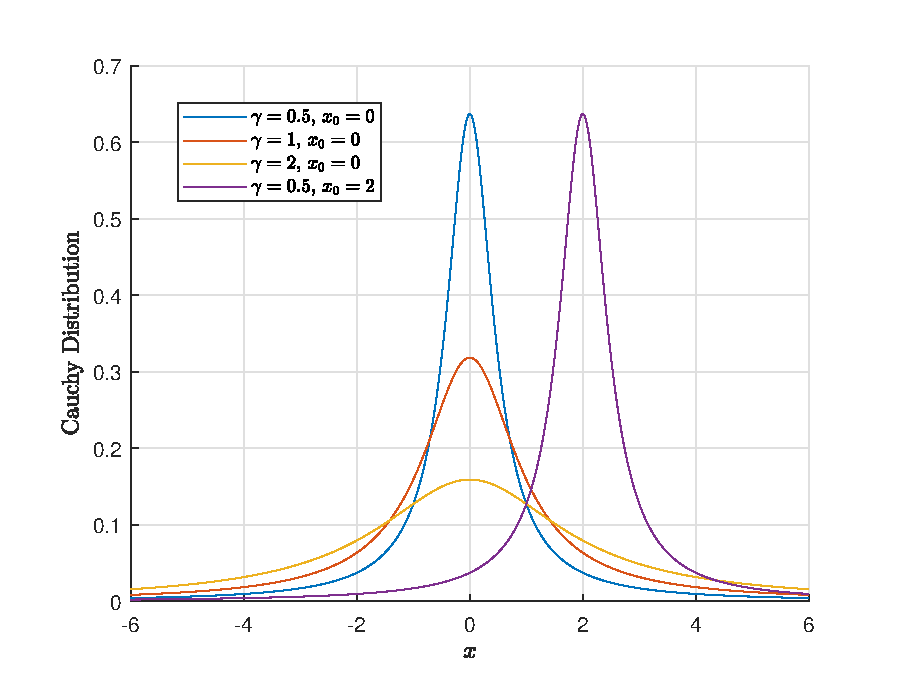
\includegraphics[width=250pt]{chapters/ch-commonly-seen-distributions/figs/cauchy_pdf.eps}
	\caption{Cauchy Distribution.} \label{fig:cauchy_pdf}
\end{figure}

From mathematics perspective, Cauchy distribution describes the ratio of two independent normal distributed random variables with mean zero. It is a useful distribution in physics.

\section{Gamma, Chi-Squared and Beta Distributions}

The $\Gamma$, $\chi^2$ and $\beta$ distributions are introduced as follows.

\subsection{The $\Gamma$ Distribution}

Gamma distribution is a continuous distribution with the following PDF
\begin{eqnarray}
  f(x) &=& \left\{\begin{array}{cc}
                    \dfrac{\beta^\alpha}{\Gamma(\alpha)}x^{k-1}e^{-\beta x} & x > 0 \\
                    0 & \textup{otherwise}
                  \end{array}\right. \label{eq:gammapdf}
\end{eqnarray}
where $\alpha>0$ and $\beta>0$ are the shape parameters (some literatures uses scale parameter $\theta = 1/\beta$ in the equation), and $\Gamma(\cdot)$ denotes the Gamma function
\begin{eqnarray}
  \Gamma(\alpha) &=& \int_{0}^{\infty}t^{\alpha-1}e^{-t}dt \nonumber
\end{eqnarray}
for $\alpha > 0$. Gamma distribution is often used to model the interval of two events in the Poisson process.

The plot of the PDF of Gamma distribution is given in Fig. \ref{fig:gamma_pdf}.
\begin{figure}
	\centering
	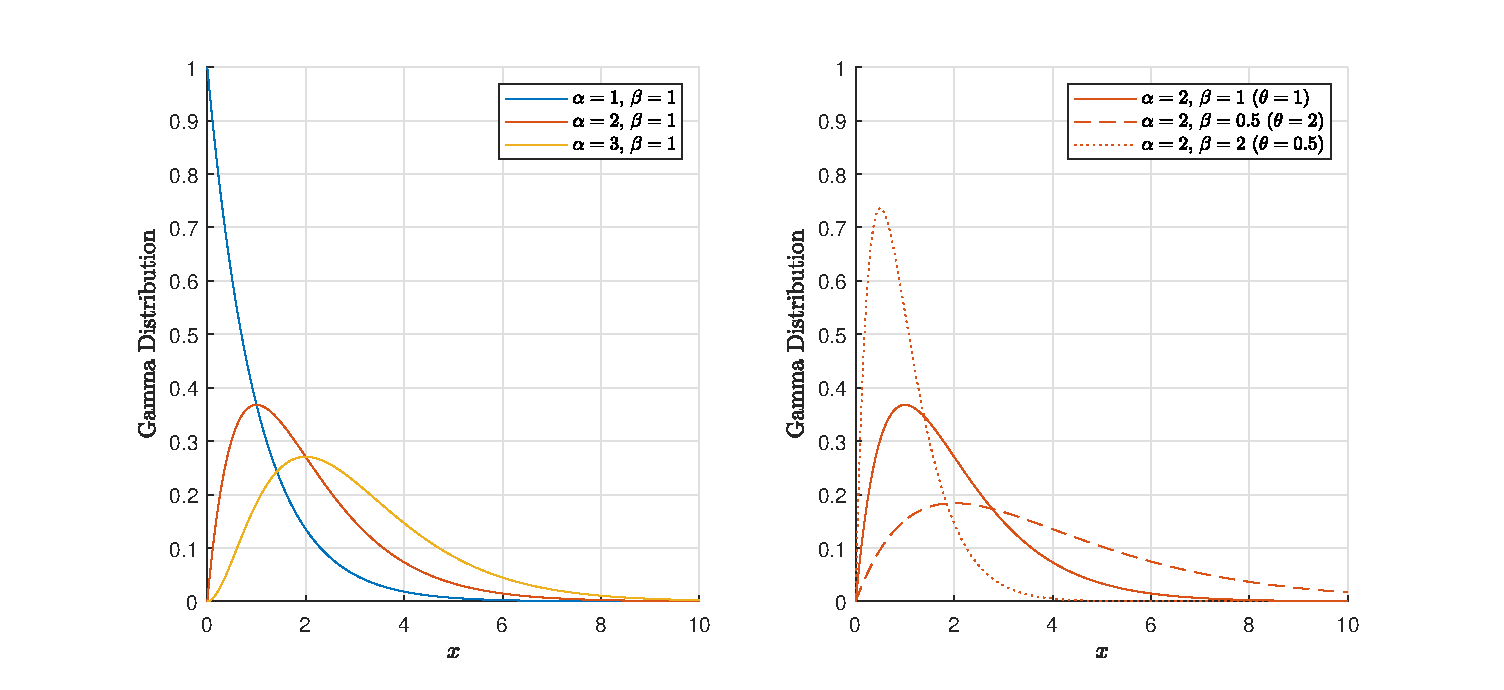
\includegraphics[width=350pt]{chapters/ch-commonly-seen-distributions/figs/gamma_pdf.eps}
	\caption{Gamma Distribution.} \label{fig:gamma_pdf}
\end{figure}

\begin{shortbox}
\Boxhead{A Little Bit about Gamma Function}

Gamma function is given by
\begin{eqnarray}
  \Gamma(\alpha) &=& \int_{0}^{\infty}t^{\alpha-1}e^{-t}dt \nonumber
\end{eqnarray}

It is clear that $\Gamma(1)=1$. If $\alpha > 1$, an integration by parts shows that
\begin{eqnarray}
  \Gamma(\alpha) &=& (\alpha-1)\Gamma(\alpha-1) \nonumber
\end{eqnarray}
Therefore, $\Gamma(n)=\Gamma(n-1)\Gamma(n-2)\ldots \times 3 \times 2 \times 1 \times \Gamma(1) = (\alpha-1)!$ for $\alpha \in \mathbb{N}^+$, with $0!=1$.

\end{shortbox}

The expectation, variance, skewness and excess kurtosis of the distribution are $\dfrac{\alpha}{\beta}$, $\dfrac{\alpha}{\beta^2}$, $\dfrac{2}{\sqrt{\alpha}}$ and $\dfrac{6}{\alpha}$, respectively.

\subsection{The $\chi^2$ Distribution}

The $\chi^2$ estimation is a special case of Gamma distribution. In \eqref{eq:gammapdf}, let $\alpha = \dfrac{r}{2}$ and $\beta=\dfrac{1}{2}$ to get the PDF of $\chi^2$ distribution as follows.
\begin{eqnarray}
  f(x) &=& \left\{\begin{array}{cc}
                    \dfrac{1}{\Gamma(r/2)2^{r/2}}x^{r/2-1}e^{-x/2} & x > 0  \\
                    0 & \textup{otherwise}
                  \end{array}\right. \label{eq:chi2pdf}
\end{eqnarray}
Equation \eqref{eq:chi2pdf} is also denoted by $\chi^2(r)$, where $r$ is known as the degrees of freedom. The plots of PDFs with different $\gamma$ are shown in Fig. \ref{fig:chi2_pdf}.
\begin{figure}
	\centering
	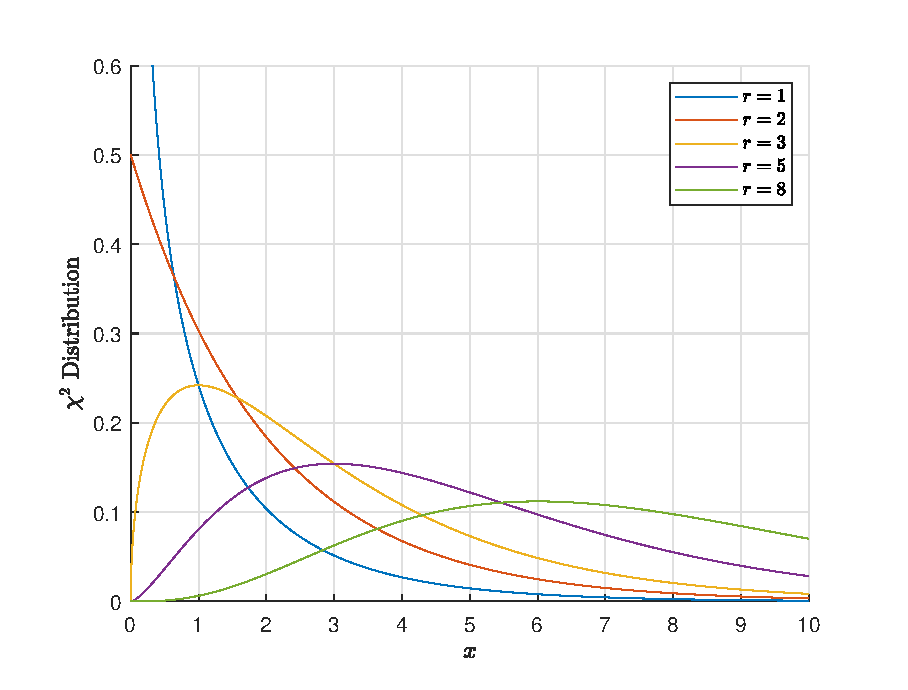
\includegraphics[width=250pt]{chapters/ch-commonly-seen-distributions/figs/chi2_pdf.eps}
	\caption{The $\chi^2$ Distribution.} \label{fig:chi2_pdf}
\end{figure}

The $\chi^2$ distribution can be used to model the sum of the squares of $r$ independent standard normal distributions, making it an important distribution is statistics, such as in outlier test. 

The expectation, variance, skewness and excess kurtosis of the distribution are $r$, $2r$, $\sqrt{\dfrac{8}{r}}$ and $\dfrac{12}{r}$, respectively.

\subsection{The $\beta$ Distribution}

Let $X_1$ and $X_2$ be two independent random variables following Gamma distributions with shape parameters $\alpha_1$ and $\alpha_2$ respectively and with $\beta = 1$ in the PDF \eqref{eq:gammapdf}. Denote $X=\dfrac{X_1}{X_1+X_2}$. In this case, $X$ would be a random variable following $\beta$ distribution whose PDF can be derived from \eqref{eq:gammapdf} and it is given by
\begin{eqnarray}
  f(x) &=& \left\{\begin{array}{cc}
                    \dfrac{\Gamma(\alpha_1 + \alpha_2)}{\Gamma(\alpha_1)\Gamma(\alpha_2)}x^{\alpha_1-1}(1-x)^{\alpha_2-1} & 0 < x < 1 \\
                    0 & \textup{otherwise}
                  \end{array}\right. \label{eq:betapdf}
\end{eqnarray}
In some literatures, notation $(a, b)$ or $(\alpha, \beta)$ are used to denote $(\alpha_1, \alpha_2)$ in \eqref{eq:betapdf}.

\section{Student's $t$-Distribution}



The zero-mean $t$-distribution PDF is given by
\begin{eqnarray}
	f(x) &=& \dfrac{\Gamma\left(\dfrac{\nu+1}{2}\right)}{\sqrt{\nu\pi}\sigma\Gamma\left(\dfrac{\nu}{2}\right)}\left(1+\dfrac{x^2}{\nu\sigma^2}\right)^{-\dfrac{\nu+1}{2}} \label{eq:tpdf}
\end{eqnarray}
where $\nu$ and $\sigma$ are known as the shape and scale parameters respectively. When $\nu\rightarrow\infty$, \eqref{eq:tpdf} reduces to normal distribution. 

Student's $t$-distribution can also be derived from normal and $\chi^2$ distributions as follows. Let $X_1$ and $X_2$ be two random variables following standard normal distribution and $\chi^2$ distribution with degree of freedom $\nu$. Let
\begin{eqnarray}
	X &=& \dfrac{X_1}{\sqrt{\dfrac{X_2}{\nu}}} \nonumber
\end{eqnarray}
then $X$ follows $t$-distribution \eqref{eq:tpdf}.

Student's $t$-distribution is famous for its heavy-tail characteristics, and it is good at emulating noise with outliers.

The expectation, variance, skewness and excess kurtosis of the $t$-distribution given by \eqref{eq:tpdf} are $0$, $\dfrac{\nu}{\nu-2}$ $(\nu>2)$, $0$ $(\nu>3)$ and $\dfrac{6}{\nu-4}$ $(\nu>4)$ respectively.

\section{$F$-Distribution}

Let $X_1$, $X_2$ be two random variables following $\chi^2$ distribution with degree of freedom $\nu_1$ and $\nu_2$ respectively. Let
\begin{eqnarray}
	X &=& \dfrac{\dfrac{X_1}{\nu_1}}{\dfrac{X_2}{\nu_2}} \nonumber
\end{eqnarray}
then $X$ follows $F$-distribution, named after R.A. Fisher.

The PDF of the $F$-distribution is given by
\begin{eqnarray}
	f(x) &=& \left\{\begin{array}{cc}
		\dfrac{\Gamma\left(\dfrac{\nu_1+\nu_2}{2}\right)}{\Gamma\left(\dfrac{\nu_1}{2}\right)\Gamma\left(\dfrac{\nu_2}{2}\right)}\nu_1^{\dfrac{\nu_1}{2}}\nu_2^{\dfrac{\nu_2}{2}}x^{\left(\dfrac{\nu_1}{2}-1\right)}\left(\nu_2+\nu_1 x\right)^{-\dfrac{\nu_1+\nu_2}{2}} & x > 0 \\
		0 & \textup{otherwise}
	\end{array}\right. \nonumber
\end{eqnarray}
where $\nu_1$, $\nu_2$ are the shape parameters of the distribution.
